%!TEX root = ../crowd_hierarchies_kdd.tex

\section{Preliminaries}
\label{sec:prelims}
In this section we provide the necessary definitions and background for formalizing the problem of crowdsourced entity extraction when considering structured domains. First, we define the notion of a structured domain, then describe the association between entities and the poset describing a structured domain. We continue by describing 
entity extraction queries and interfaces over structured domain, along with the response and cost model for these queries. Finally, we define the problem of {\em budgeted crowd entity extraction} over {\em structured domains} that seeks to maximize the number of extracted entities under budget constraints and present an overview of our proposed framework.


\subsection{Structured Data Domain}
\label{sec:data-domain}

Let $\domain$ be a data domain described by a set of discrete attributes $\attributes = \{A_1, A_2, \dots, A_d\}$. Let $dom(A_i)$ denote the domain of each attribute $A_i  \in \attributes$. We consider domains where each attribute $A_i$ can also be hierarchically organized. \iftr For example, consider the Eventbrite domain introduced in \Cref{sec:challenges}. The data domain $\domain$ corresponds to all events and the attributes describing the entities in $\domain$ are $\attributes = \{$``Event Type'', ``Location'', ``Date''$\}$. \Cref{fig:eventsdomain} shows the hierarchical organization of each attribute.

\begin{figure}[h]
	\begin{center}
	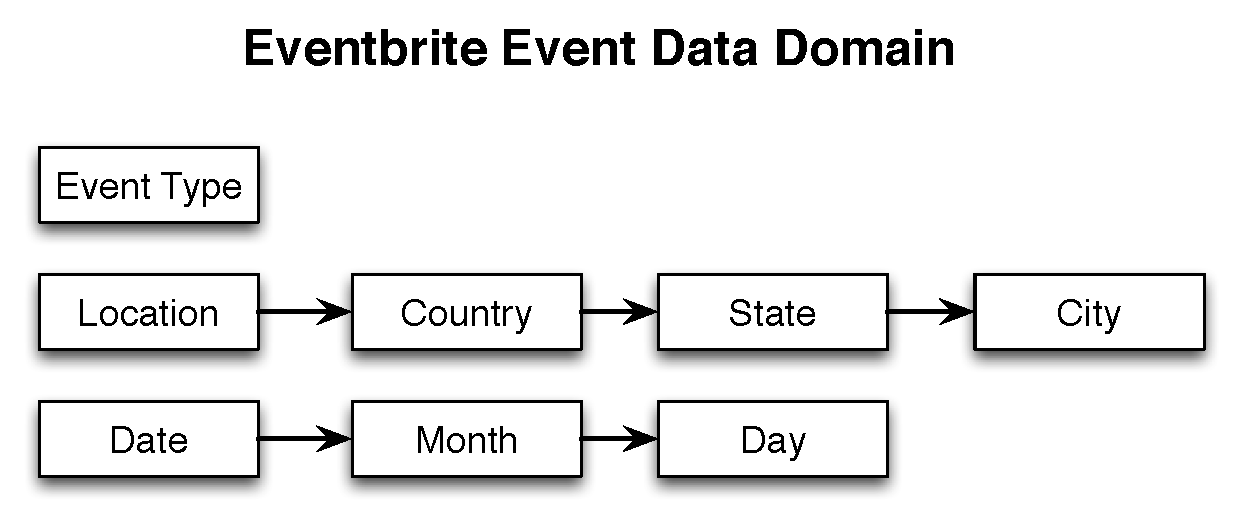
\includegraphics[clip,scale=0.33]{figs/eventsDomain.eps}
	\vspace{-10pt}
	\caption{The attributes describing the Eventbrite domain and the hierarchical structure of each attribute.}
	\label{fig:eventsdomain}
	\end{center}
	\vspace{-20pt}
\end{figure}
\fi
\ifpaper
For Eventbrite, introduced in \Cref{sec:intro}, the entities in the data domain $\domain$ correspond to events. The attributes describing the entities in $\domain$ are $\attributes = \{$``Event Type'', ``Location'', ``Date''$\}$, with ``Location'' and ``Date'' being hierarchically organized.
\fi
The domain $\domain$ can be viewed as a {\em poset}, i.e., a partially ordered set, corresponding to the cross-product of all available hierarchies\footnote{Note that $\domain$ is not a lattice since there is no unique infimum.}. Part of the poset corresponding to the previous example is shown in \Cref{fig:eventslattice}. We denote the poset for a domain $\domain$ as $\hierarchy$. As shown in \Cref{fig:eventslattice}, nodes in the poset me correspond to configurations where only a subset of the attributes in $\attributes$ are specified while others are allowed to take any value. For example the root of the poset $\{\}$ has no specified attributes allowing for queries of the form ``list an event''. Nodes at lower levels, such as $\{X1\}$ and $\{C1\}$, correspond to queries where the event type and location are specified respectively. 

\begin{figure}[h]
	\begin{center}
	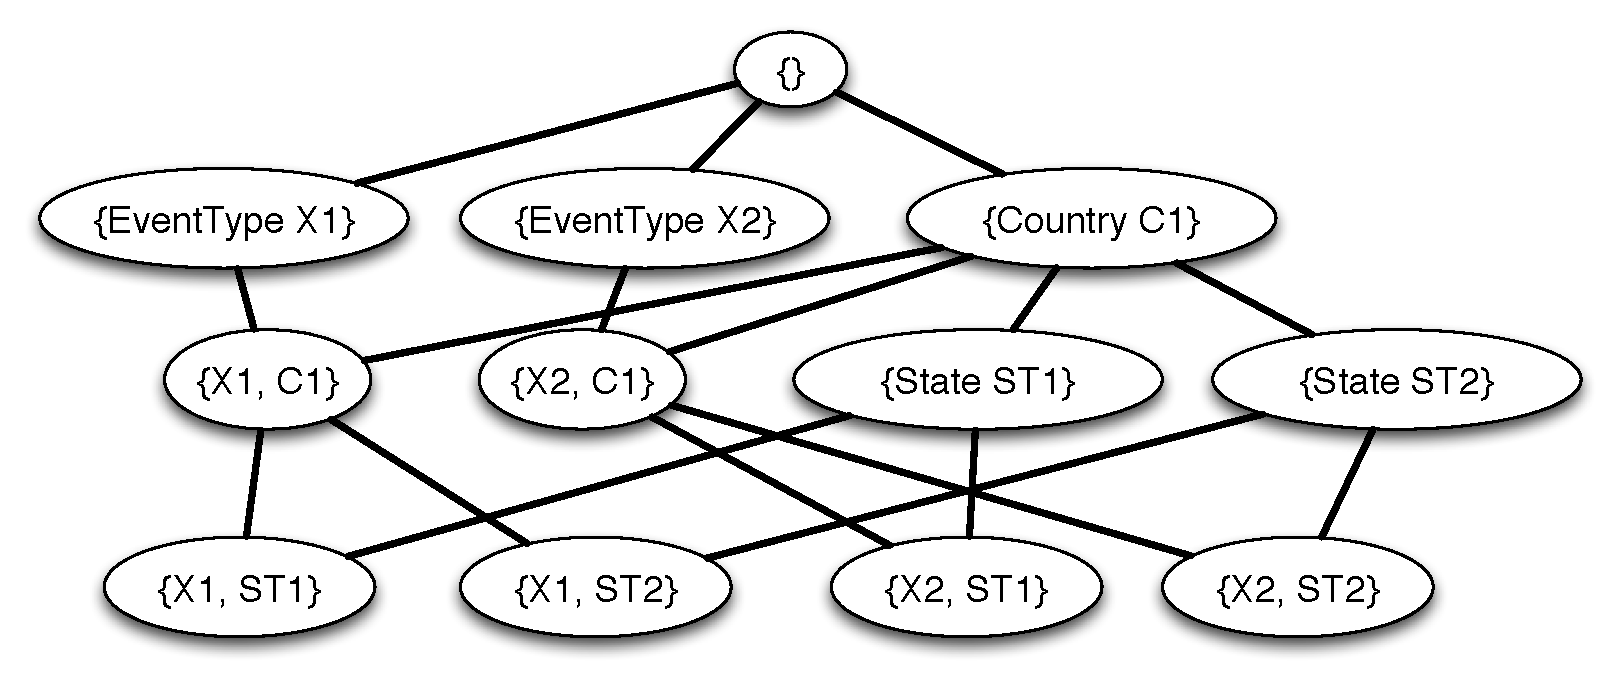
\includegraphics[clip,scale=0.3]{figs/eventsExLattice.eps}
	\caption{Part of the poset defining the entity domain for Eventbrite.}
	\label{fig:eventslattice}
	\end{center}
\end{figure}

\subsection{Entities and Entity Extraction Queries}
\label{sec:queries}

\stitle{Entities.} Our goal is to extract entities that belong to the domain $\domain$. We assume that each entity $e$ can be uniquely associated with one of the leaf nodes in the hierarchy $\hierarchy$; that is, there is a unique combination of attribute values $A_1, \ldots, A_d$ characterizing each entity. For example, in Eventbrite, each entity (here, a local event) is of a specific type, takes place in a specific city, and on a specific day. Our techniques are also applicable when entities are underspecified, i.e., only a subset of the attributes in $\attributes$ are specified, but we focus on the former case for simplicity.

\stitle{Queries.} Next, we introduce the notion of {\em generalized extraction queries} that can be issued against crowd workers. We require that a query $q^v$ is associated with a node $v \in \hierarchy$; that is a query contains predicates that correspond to zero or more attribute in $\attributes$ and the predicates correspond to the value combination for $\attributes$ associated with $v$. For example, if we consider the poset shown in \Cref{fig:eventslattice} a query for node $\{X1\}$ has a predicate $EventType = X1$. Hence, workers are required to provide entities, here, events, that satisfy this predicate, i.e., they are of type $X1$.

Given a query $q^v$ associated with node $v \in \hierarchy$, we consider three different further configurations for  extracting entities from the crowd: The first configuration corresponds to {\em single entity queries} where workers are required to provide only ``one more'' entity matching the predicates of the query. Considering the Eventbrite example introduced in the previous section, an example of a single entity query would be asking a worker to provide ``a concert in New York'', where the predicates are $\mathsf{EventType = concert}$ and $\mathsf{State = New York}$. The second configuration corresponds to {\em queries of size k} where workers are asked to provide up to $k$ distinct entities for a query $q^v$. Finally, the last configuration corresponds to {\em exclude list queries}. Here,  workers are additionally provided with a list $E$ of $l$ entities that have already been extracted and are required to provide up to $k$ distinct entities that are not present in the exclude list. It is easy to see that the last configuration generalizes the previous two. Therefore, in the remainder of the paper, we will only consider queries using the third configuration. We refer to these queries as {\em generalized}. To describe a generalized query, we will use the notation $q^v(k,E)$ denoting a query of size $k$ accompanied with an exclude list $E$ of length $l$ and associated with node $v \in \hierarchy$. We will denote the configuration characterizing the query as $(k,l,v)$. 

\stitle{Query Response.} Given a query $q^v(k, E)$ issued at a node $v \in \hierarchy$, a human worker gives us $k$ distinct entities that belong to the domain $\domain$, match the query predicates and are not present in $E$. Furthermore, we consider a querying interface that asks human workers to not only list entities but to also provide,  for each entity, the values to the remaining attributes in $\attributes$ that are not specified in the predicates of $q$. For example, if our query is ``list one concert in Manhattan, New York'', with $k = 1, E = \emptyset$, the human worker gives us one concert in Manhattan, New York, but also gives us the day on which the concert will take place (here, the missing, unspecified attribute) and potentially the type of concert, i.e,. rock concert. If the query is ``a concert in the US'', with $k = 1, E = \emptyset$, the human worker gives us one concert in the US, but also gives the day on which the concert will take place, as well as the specific city. If less than $k$ entities are present in the underlying population, workers have the flexibility to report either an empty answer or a smaller number of entities (\Cref{sec:excludelist}).

While the reader may wonder if getting additional attribute values for entities is necessary, we note that this information allows us to assign an extracted entity to all nodes in $\hierarchy$ the entity belongs to; without this, it is difficult to effectively collect information about the underlying entity population associated with each node in the poset. Furthermore, we find that in most practical applications, it is useful to get the values of the missing attributes to organize and categorize the extracted entities better. Similar query interfaces that ask users to fully specify the attributes of entities have been proposed in recent literature~\cite{quinn:2014}. 

\ifpaper \stitle{Detecting Duplicate Entities.} Naturally, we expect workers to provide us with duplicate extractions and erroneous extractions. 

Finally, answers are expected to be duplicated across workers, who may also provide an entity incorrectly. Resolving duplicates during extraction is crucial as they are used to estimate the completeness of extracted entities, and thus, reason about the gain of additional queries. Standard entity resolution techniques~\cite{getoor:kdd13} can be used to address this problem. Nevertheless entity resolution is an orthogonal problem and not the focus of this paper. \fi

\iftr
Finally, answers are expected to be duplicated across workers, who may also specify or extract an entity incorrectly. Resolving duplicate entities during extraction is crucial as this information is later used to estimate characterize the completeness of extracted entities, and thus, reason about the gain of additional queries.  Extraction errors can be resolved by leveraging the presence of duplicate information and by applying de-duplication and entity resolution techniques. At a high-level one can use an entity resolution or string similarity (e.g., jaccard coefficient) algorithm to identify duplicate entities. Furthermore, the additional attributes for each entity, can be used to further ascertain similarity of entities. We refer the user to Getoor and Machanavajjhala~\cite{getoor:kdd13} for an overview of entity resolution techniques. Finally, standard truth discovery techniques can be used to identify the correct attribute values for entities. Nevertheless entity resolution and truth discovery are orthogonal problems and not the focus of this paper. In our experiments on real datasets, we found that there were no cases where humans introduced errors to the attribute values of extracted entities. Only minor errors (e.g., misspelled entity names) were detected and fixed manually. \fi

\stitle{Query Cost.} In a typical crowdsourcing marketplace, tasks have different costs based on their difficulty. Thus, crowdsourced queries of different difficulties should also exhibit different costs. We assume we are provided with a cost function $c(\cdot)$ that obeys the following properties:  (a) given a query with fixed size its cost should increase as the size of its exclude list is increasing, and (b) given a query with a fixed exclude list size its cost should increase as the number of requested answer increases. These are fixed upfront by the interface-designer based on the amount of work involved.

\subsection{Crowdsourced Entity Extraction}
\label{sec:extraction}
The basic version of {\em crowdsourced entity extraction}~\cite{trushkowsky:2013} seeks to extract entities that belong to $\domain$, by simply using repeated queries at the root node, with $k = 1, E = \emptyset$. When considering large entity domains, one may need to issue a series of entity extraction queries at multiple nodes in  $\hierarchy$ --- often overlapping with each other --- so that the entire domain is covered. Issuing queries at different nodes ensures that the coverage across the domain will be maximized. 

We let $\pi$ denote a {\em querying policy}, i.e., a chain of queries at different nodes in $\hierarchy$. Notice that multiple queries $q(k,E)$ can be issued at the same node. Let $C(\pi)$ denote the overall cost, in terms of monetary cost of a querying policy $\pi$. We define the gain of a querying policy $\pi$ to be the total number of unique entities, denoted by $\uentities(\pi)$ extracted when following policy $\pi$. Thus, there is a natural tradeoff between the gain (i.e., the number of extracted entities) and the cost of policies. 

Here, we require that the user will {\em only} provide a monetary budget $\tau_c$ imposing a constraint on the total cost of a selected querying policy, and optimize over all possible querying policies across different nodes of $\hierarchy$. Our goal is to identify the policy that maximizes the number of retrieved entities under the given budget constraint. More formally, we define the problem of budgeted crowd entity extraction as follows:

\begin{problem}[Budgeted Crowd Entity Extraction] \ \\
Let $\domain$ be a given entity domain and $\tau_c$ a monetary budget on the total cost of issued queries. The Budgeted Crowd Entity Extraction problem seeks to find a querying policy $\pi^*$ using queries $q(k,E)$ over nodes in $\hierarchy$ that maximizes the number of unique entities extracted $\uentities(\pi^*)$ under the constraint $C(\pi^*) \leq \tau_c$.
\end{problem}
The optimal policy not only specifies the nodes at which queries will be executed but also the size and exclude list of each query.

The cost of a querying policy $\pi$ is defined as the total cost of all queries issued by following $\pi$. We have that $C(\pi) = \sum_{q \in \pi} c(q)$ where the cost of each query $q$ is defined according to a cost model specified by the user. Computing the total cost of a policy $\pi$ is easy. However, the gain $\uentities(\pi)$ of a policy $\pi$ is unknown as we do not know in advance the entities corresponding to each node in $\hierarchy$, and hence, needs to be estimated, as we discuss next. 

The problem of budgeted crowd entity extraction is an instance of a generalization of the {\em stochastic knapsack problem}~\cite{kosuch,steinberg} where each item has a deterministic cost (weight) but a stochastic profit. The stochastic knapsack problem is known to be NP-hard and so is the budgeted crowd entity extraction problem.

\subsection{Underlying Query Response Model}
\label{sec:sampling}
To reason about the occurrence of entities as response to specific queries, we need an underlying query response model. Our query response model is based on the notion of {\em popularity}.
\ifpaper We assume that each underlying entity has a {\em fixed, unknown popularity value} with respect to crowd workers. Given a query $q(1, \emptyset)$, asking for one entity without using an exclude list, the probability that we will get entity $e$ that satisfies the constraints specified by $q$ is nothing but the popularity value of $e$ divided by the popularity value of all entities $e'$ that also satisfy the constraints in $q$. As an example, if there are only two entities $e_1, e_2$ that satisfy the constraints specified by a given query $q_1$, with popularity values $3$ and $2$,
then the probability that we get $e_1$ on issuing a query $q_1(1, \emptyset)$ is 3/5. If an exclude list $E$ is specified, then the probability that we will get an entity $e \notin E$ is the popularity value of $e$ divided by the popularity values of all entities $e' \notin E$ also satisfying the constraints specified by $q$. {\bf We do not assume that all workers follow the same popularity distribution}. Rather the overall popularity distribution can be seen as an average of the popularity distributions across all workers.

Since workers are asked to provide a limited number of entities as response to a query, each entity extraction query can be viewed as taking a random sample from an unknown population of entities. In the rest of the paper, we will refer to the distribution characterizing the popularities of entities in a population of entities as the {\em popularity distribution} of the population. We note that this is equivalent to the underlying assumption in the species estimation literature~\cite{chao:1992} (\Cref{sec:gainestimators}). Then, estimating the gain of a query $q(k,E)$ at a node $v \in \hierarchy$ is equivalent to estimating the number of new entities extracted by taking additional samples from the population of $v$ given all the retrieved entities (i.e., {\em running sample}) associated with node $v$~\cite{trushkowsky:2013}. Due to the structure of the poset we may retrieve entities for a node when issuing queries at other nodes. We discuss this form of {\em indirect sampling} in the extended version of this paper~\cite{crowdgatherfull}. 
\fi
\iftr
\stitle{Popularities.} We assume that each underlying entity has a {\em fixed, unknown popularity value} with respect to crowd workers. Given a query $q(1, 0)$, asking for one entity and using an exclude list of size $0$, the probability that we will get entity $e$ that satisfies the constraints specified by $q$ is nothing but the popularity value of $e$ divided by the popularity value of all entities $e'$ that also satisfy the constraints in $q$. As an example, if there are only two entities $e_1, e_2$ that satisfy the constraints specified by a given query $q_1$, with popularity values $3$ and $2$,
then the probability that we get $e_1$ on issuing a query $q_1(1, 0)$ is 3/5. 
If an exclude list $S$ is specified, then the probability that we will get an entity $e \notin S$ is the popularity value of $e$ divided by the popularity values of all entities $e' \notin S$ also satisfying the constraints specified by $q$. Note that, we {\bf do not assume that all workers follow the same popularity distribution}. Rather the overall popularity distribution can be seen as an average of the popularity distributions across all workers.

Thus, since workers are asked to provide a limited number of entities as response to a query, each entity extraction query can be viewed as taking a random sample from an unknown population of entities. In the rest of the paper, we will refer to the distribution characterizing the popularities of entities in a population of entities as the {\em popularity distribution} of the population. We note that this is equivalent to the underlying assumption in the species estimation literature~\cite{chao:1992} (\Cref{sec:gainestimators}).

% We assume that the underlying entities exhibit different {\em popularity levels} with respect to crowd workers. These popularity levels can be formally defined using the notion of a probability distribution. In particular, the probability that an entity will appear as part of a query result depends on its {\em popularity} relative to the overall entity population. The popularity of an entity for a query $q$ is defined as the probability that this entity will appear in a query $q(1,0)$, i.e., a query asking for one entity from the population and using an exclude list of size zero. Since workers are asked to provide a limited number of entities as response to a query, each entity extraction query can be viewed as taking a random sample from an unknown population of entities. In the remainder of the paper, we will refer to the distribution characterizing the popularities of entities corresponding to a population as the {\em popularity distribution} of the population. 

Then, estimating the gain of a query $q(k,l)$ at a node $v \in \hierarchy$ is equivalent to estimating the number of new entities extracted by taking additional samples from the population of $v$ given all the retrieved entities by past samples associated with node $v$~\cite{trushkowsky:2013}. 

\stitle{Samples for a Node.} When extracting entities,  the retrieved entities for a node $v$ can correspond to two different kinds of samples: (i) those that were extracted by considering the {\bf entire population} corresponding to node $v$ (ii) and those that we obtained by sampling {\bf only a part of the population} corresponding to $v$. Samples for a node $v$ can be obtained either by querying node $v$ or by indirect information flowing to $v$ by queries at other nodes. We refer to the latter case as {\em dependencies across queries}. 
\begin{figure}[h]
	\begin{center}
	\vspace{-10pt}
	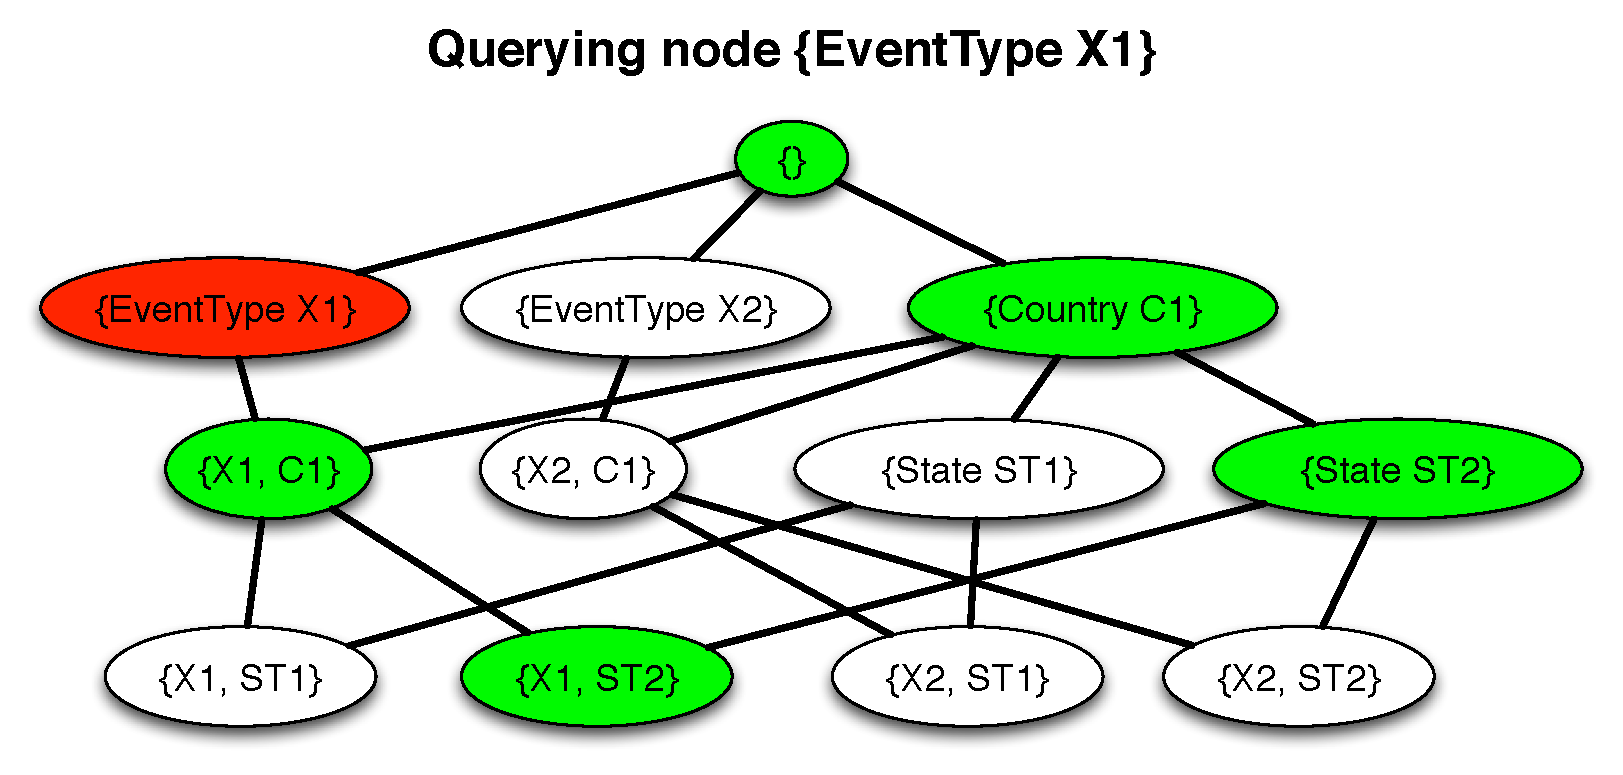
\includegraphics[clip,scale=0.3]{figs/exampleQuery.eps}
	\caption{An example query that extract an entity sample from the red node. The nodes marked with green correspond to the nodes for which indirect entity samples are retrieved.}
	\label{fig:query}
	\vspace{-10pt}
	\end{center}
	\vspace{-5pt}
\end{figure}

We use an example considering the poset in \Cref{fig:eventslattice}, to illustrate these two cases. The example is shown in \Cref{fig:query}. Assume a query $q(k,0)$ issued against node \{EventType X1\}. Assume that the query result contains entities that correspond only to node \{X1,ST2\}. The green nodes in \Cref{fig:query} are nodes for which samples are obtained indirectly without querying them. Notice, that all these nodes are ancestors of \{X1,ST2\}. Analyzing the samples for the different nodes we have:
\squishlist
\item The samples corresponding to nodes \{X1, C1\} and \{X1,ST2\} were obtained by considering their {\em entire population}. The reason is that node \{EventType X1\} is an ancestor of both and the entity population corresponding to it fully contains the populations of both \{X1,C1\} and \{X1,ST1\}. 
\item The samples corresponding to nodes \{ \}, \{Country C1\} and \{State ST2\} were obtained by considering only part of their population. The reason is that the population of node \{EventType X1\} does not fully contain the populations of these nodes. 
\squishend

Samples belonging to both types need to be considered when estimating the gain of a query at a node in $v \in \hierarchy$. To address this issue we merge the extracted entities for each node in $\hierarchy$ into a single sample and treat the unified sample as being extracted from the entire underlying population of the node. As we discuss later in \Cref{sec:solving} we develop querying strategies that traverse the poset $\hierarchy$ in a top-down approach, hence, the number of samples belonging in the first category, i.e., samples retrieved considering the entire population of a node, dominates the number of samples retrieved by considering only part of a node's population. Moreover, it has been shown by Hortal et al.~\cite{hortal2006evaluating} that several of the techniques that can be used to estimate the gain of a query (see \Cref{sec:gainestimators}) are insensitive to differences in the way the samples are aggregated.
\fi
\subsection{Framework Overview}
\label{sec:framework}
We view the optimization problem described in \Cref{sec:extraction} as a multi-round adaptive optimization problem where at each round we solve the following subproblems: 
\squishlist 
\item \textbf{Estimating the Gain for a Query.} For each node in $v \in \hierarchy$, consider the retrieved entities associated with $v$ and estimate the number of new unique entities that will be retrieved if a new query $q(k,E)$ is issued at $v$. This needs to be repeated for different query configurations. 
\item \textbf{Detecting the Optimal Querying Policy.} Using the gain estimates from the previous problem as input, identify the next (query configuration, node) combination so that the total gain across all rounds is maximized with respect to the given budget constraint. When identifying the next query we do not explicitly optimize for the exclude list to be used. We rather optimize for the exclude list size $l$. Once the size is selected, the exclude list is constructed in a randomized fashion. We elaborate more on this design choice in \Cref{sec:heuristic}.
\squishend
Our proposed framework iteratively solves the aforementioned problems until the entire budget is used. \iftr \Cref{fig:framework} shows a high-level diagram of our proposed framework.
% Throughout our framework, we assume that after issuing a query against the crowd, the retrieved answers can be associated with all relevant nodes across all attribute hierarchies, i.e., a worker will provide all the attribute values describing a reported entity. Dealing with incomplete information about entities is not the main focus of this paper and is part of the future work preposed in \Cref{sec:conclusions}.

\begin{figure}
	\begin{center}
	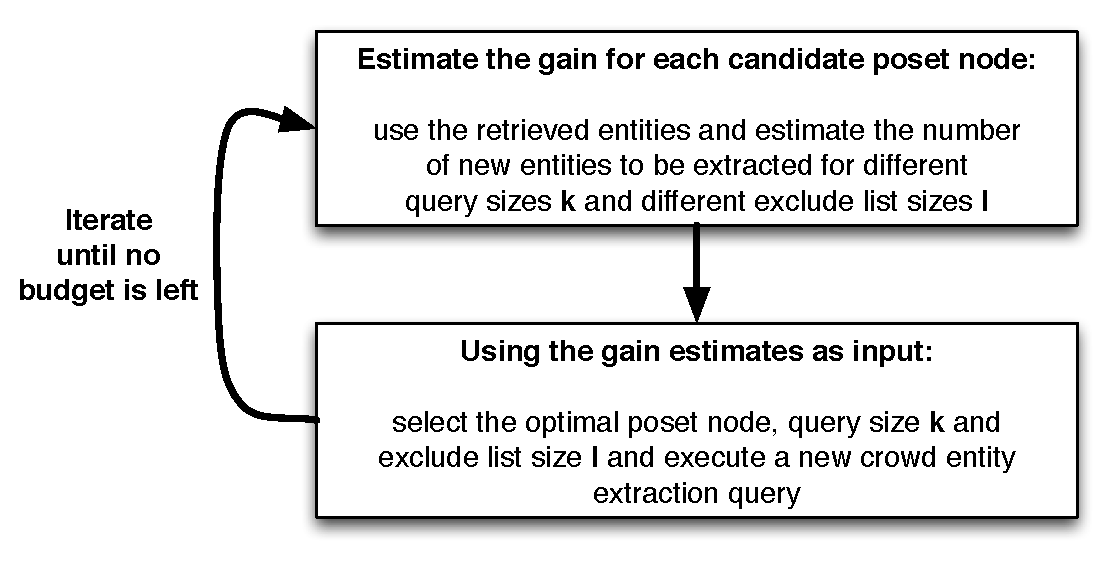
\includegraphics[clip,scale=0.43]{figs/framework.eps}
	\vspace{-10pt}
	\caption{Framework overview for budgeted entity extraction.}
	\label{fig:framework}
	\end{center}
	\vspace{-20pt}
\end{figure}
\fi